\chapter{Introduction}

\section{Contexte}
La précision du positionnement intérieur reste quelque chose de très important, car il peut être utile dans plusieurs domaines comme : la gestion de stocks, la localisation de personnes âgées dans des homes, la localisation de personnes pour la surveillance, etc.

Les systèmes de localisation basés sur GPS souffrent de la détérioration de la précision et sont presque indisponibles dans les environnements intérieurs. Pour les environnements intérieurs, de nombreuses technologies de systèmes de positionnement ont été conçues sur la base de la vision, de la détection infrarouge ou ultrasonore, des champs magnétiques de la terre, des accéléromètres / gyromètres, des balises BLE ou de la communication WiFi. Bien que la création de ces nouvelles applications ait été couronnée de succès, le coût de ces récepteurs, leur consommation d’énergie et leur limitation aux environnements extérieurs excluent de nombreuses applications.

La Figure \ref{fig:MethodePos} montre un graphique comparatif de la précision de positionnement concernant différentes technologies \cite{INPOS}. Ce graphique montre qu'un système utilisant la vision apporte une grande précision. Mais, il peut poser des problèmes dans certaines applications où il serait nécessaire de mettre beaucoup de caméras et cela implique souvent des traitements assez complexes. En comparaison, un système à ultrason qui est un peu comparable à un système infrarouge est meilleur marché. Il est également nécessaire de placer un grand nombre de capteurs selon les utilisations. Concernant les systèmes RFID, ils ont une portée très courte qui se limite à quelques mètres et la précision est dégradée par rapport aux systèmes précédents. Les deux derniers systèmes qui sont les réseaux sans fil (Bluetooth et WLAN) possèdent beaucoup d'avantages, car ils sont largement répandus et possèdent une bonne couverture. Un gros inconvénient de ces deux technologies est qu'elles sont gourmandes en énergie et ne peuvent pas fonctionner sur batterie.

\begin{figure}[htp]
 \begin{center}
  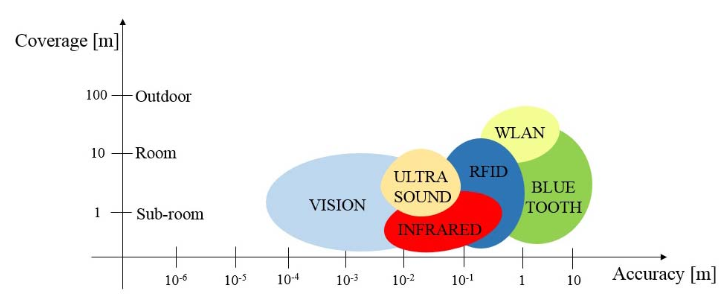
\includegraphics[scale=0.7]{figures/MethodePos.png}
  \caption{État de l'art des différentes méthodes de positionnement intérieur \cite{INPOS}}
  \label{fig:MethodePos} %% NOTE: always label *after* caption!
 \end{center}
\end{figure}

La localisation avec LoRa est une possibilité séduisante et probablement l'une des meilleures candidates pour le positionnement intérieur. Le faible coût des infrastructures et des noeuds finaux ainsi que la disponibilité pourraient permettre de nombreuses nouvelles applications. Il n’est donc pas surprenant que les chercheurs et les entités commerciales se soient mis au travail sur ce problème au cours des derniers mois. Cependant, plusieurs défis restent à relever pour qu'un tel système devienne pratique.

LoRa peut également être utilisée pour un positionnement intérieur. À ce jour, très peu d’expériences sont disponibles pour la conception de tels systèmes et c'est pourquoi il est nécessaire d'effectuer différentes études (dont ce travail) afin de connaitre la précision qui peut être atteinte. Un autre aspect très important qui fait de la technologie LoRa est une très bonne candidate pour du positionnement intérieur est sa très faible consommation. 

%La portée en milieu rural est d'environ 15km alors qu'elle est de 5km dans un milieu urbain cela grâce à la bonne sensibilité du récepteur (-130dBm). Sagemcom a obtenu de bons résultats au niveau de la précision qui est d’environ quatre mètres comme indiqué dans le document cité \cite{ML_indoor}. 

L’objectif général de ce projet est d'étudier diverses technologies d'apprentissage (Machin Learning) permettant d'améliorer la précision de la localisation en intérieur sur la base de la technologie LoRa et en utilisant le mode "ranging" qui permet de mesurer des temps de vol. 

\section{Aspect novateur}
Ce travail d'approfondissement va permettre d'évaluer une nouvelle approche pour effectuer du positionnement intérieur. En s'appuyant sur les capacités étendues des nouveaux circuits intégrés LoRa, ce projet développera et déploiera un système de localisation capable d'améliorer la précision de la position atteinte par les systèmes de localisation basés sur LoRa existants et reposants sur des mécanismes TDOA ou de "ranging". À cette fin, une exploration et une comparaison des différentes techniques "machine learning/deep learning" pour l'amélioration de la précision du positionnement basé sur le "fingerprinting" seront effectuées.

L'aspect novateur du projet est d'intégrer au système de positionnement basé sur LoRa un mécanisme d'apprentissage de la position afin d'augmenter la précision du positionnement en intérieur. 

\section{Structure du rapport}
Ce rapport va décrire dans un premier temps l’état de l’art des techniques à utiliser, en particulier les systèmes de localisation intérieurs basés sur des techniques d’apprentissage. 

Toute la partie concernant la prise de mesures pour obtenir des données sera expliquée afin de comprendre la mise en place et pouvoir la reproduire. Cette étape est très importante dans le projet, car elle va permettre d'évaluer le système. Pour se faire, un plan de mesure a été mis en place ainsi qu'une description du matériel à utiliser. Une brève explication du logiciel de prise de mesure est également présentée afin de comprendre comment les données sont récupérées et structurées.

Ensuite, basé sur les études, le choix de l'algorithme sera détaillé ainsi que son implémentation. La présentation de quelques résultats intéressants sera également détaillée en fin de rapport.  

Finalement, une perspective pour le futur sera donnée afin de pouvoir poursuivre le travail et aller plus loin dans l'analyse des données et l'apprentissage avec un algorithme de régression plutôt que de classification.

%\todo{Compléter cette partie en fin de rapport quand la structure est définie}

%\begin{enumerate}
% \item Etudier l’état de l’art des techniques à utiliser dans le cadre du projet, en particulier les systèmes de localisation indoor basés sur des techniques d’apprentissage, et réunir une documentation (env. 20% effort)
% \item Définir un plan des tests à effectuer.
% \item Définir les procédures de test
% \item Définir le setup pour la collecte de données de localisation
% \item Prise en main de l’environnement de développement pour les phases de training et du test de la technique d’apprentissage retenue (e.g., PyTorch).
% \item Implémentation de la solution ML retenue.
% \item Tester le système selon le protocole préétabli.
% \item Faire des propositions pour améliorer les performances de l’algorithme et, si possible, les implémenter.
%\end{enumerate}


%\begin{enumerate}
% \item fgfd
% \item gdgfd
%\end{enumerate}


%\begin{figure}[H]
% \begin{center}
%  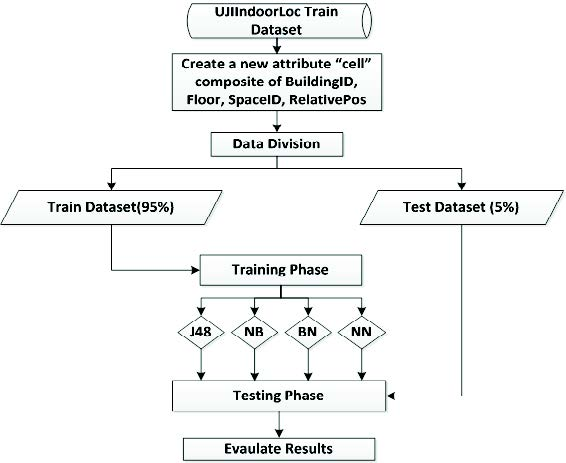
\includegraphics[scale=1]{figures/newattribute.jpg}
%  \caption{The new attribute “cell” construction phase}
%  \label{fig:newAttribute} %% NOTE: always label *after* caption!
% \end{center}
%\end{figure}



